\documentclass{psu-dissertation}
% Put your own packages and macros in preamble.tex.
% Your own packages and macros. The class already loads fontspec, newtxmath,
% geometry, setspace, fancyhdr, titlesec, tocloft, graphicx, booktabs,
% caption, natbib, and hyperref.
\usepackage{amsmath}
\graphicspath{{figures/}}

% Replace these placeholders before submitting the dissertation.
% Use \\ inside \title for a manual line break; \texorpdfstring keeps the PDF
% metadata clean, e.g. \title{First Line\texorpdfstring{\\}{ }Second Line}.
\title{Enter Your Title Here}
\author{Enter Your Name}
\graduateMajor{Enter your Graduate Major}
\degree{Doctor of Philosophy}
\graduationDate{Enter your Graduation Month and Year}
\copyrightYear{2026}
% The copyright line is optional. Uncomment to omit it:
% \showcopyrightfalse


\begin{document}
\frontmatter
\maketitle
\begin{committee}
% \committeeMember{Name}{Title(s)}{Committee role(s)}
% Do not use designations such as "Ph.D." or "Dr." for committee names.
% Add/remove members as needed. Use \\ for multiple titles or roles.
\committeeMember{Professor's Name}
  {Title(s)}
  {Dissertation Advisor\\Chair of Committee}
\committeeMember{Professor's Name}{Title}{}
\committeeMember{Professor's Name}{Title}{}
\committeeMember{Professor's Name}{Title}{}
\committeeMember{Professor's Name}
  {Title(s)}
  {Head of the Department or Director of Graduate Studies}
\end{committee}

\frontchapter*{ABSTRACT}

Enter text here.

\dissertationContents
\dissertationFigures % Remove if the dissertation has no figures.
\dissertationTables  % Remove if the dissertation has no tables.
\frontchapter{ACKNOWLEDGMENTS}

% If you have received federal funding, you must include an acknowledgment in
% this section. List all relevant award numbers and include the disclaimer
% below, naming the awarding agency(ies).
Enter text here.

This material is based upon work supported by the [awarding agency] under
Award No.~[number].
Any opinions, findings, and conclusions or recommendations expressed in this
publication are those of the author(s) and do not necessarily reflect the
views of the [name(s) of awarding agency(ies)].

% Optional front matter can follow, for example:
% \frontchapter{LIST OF ABBREVIATIONS}
% \frontchapter{DEDICATION}

\mainmatter
\chapter{Replace with Title}
\label{ch:chapter1}

Please remove this instructional text and replace it with your work.

Text in the body of your work may be single, double, or one-and-a-half
spaced. This template uses double spacing (set by \verb|\doublespacing| in
\texttt{psu-dissertation.cls}).

Chapter headings use \verb|\chapter|. Subheadings begin with \verb|\section|
and go in numerical order through \verb|\subsection| and
\verb|\subsubsection|.

\section{Replace with subheading}

\subsection{Replace with subheading}

\subsubsection{Replace with subheading}

\section{Page Breaks}

Each chapter starts on a new page automatically, so no manual page or
section breaks are needed. In the Word template, these breaks are shown with
the Show/Hide~\P{} button (\autoref{fig:show-hide}).

\begin{figure}[htbp]
  \centering
  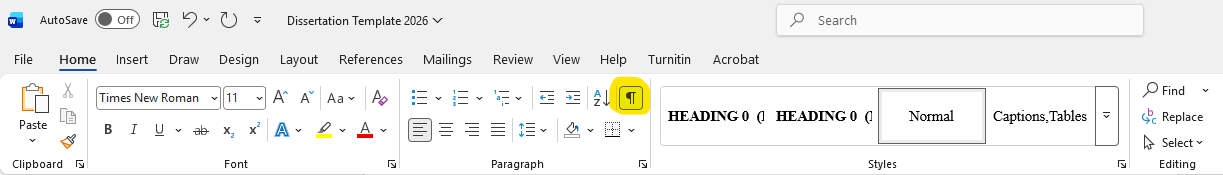
\includegraphics[width=0.5\textwidth]{show-hide}
  \caption{Show/Hide \P}
  \label{fig:show-hide}
\end{figure}

\chapter{Replace with Title}
\label{ch:chapter2}

Please remove all sample text, including figures and tables, and replace it
with your work. Below are some examples of figures, tables, equations, and
citations.

\section{Figure Example}

All figures and tables in your work must be properly referenced in the text.
For example, below you will find a picture of the Nittany Lion
(Fig.~\ref{fig:nittany-lion}). All figure captions go directly beneath the
figure.

\begin{figure}[htbp]
  \centering
  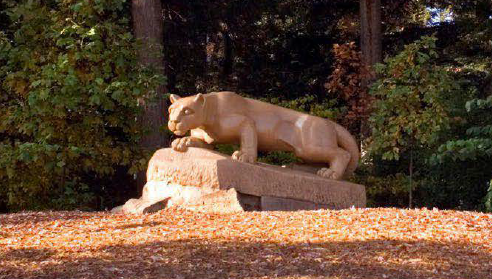
\includegraphics[width=0.6\textwidth]{nittany-lion}
  \caption{The Nittany Lion}
  \label{fig:nittany-lion}
\end{figure}

\section{Table Example}

All table captions go directly above the table. Please see the example
(Table~\ref{tab:front-matter}) below.

\begin{table}[htbp]
  \centering
  \caption{Front Matter Requirements}
  \label{tab:front-matter}
  \setlength{\tabcolsep}{5pt}
  \begin{tabular}{lll}
    \toprule
    \tableheading{Page} & \tableheading{Required} & \tableheading{Visible Page Number} \\
    \midrule
    Title Page & Mandatory & No \\
    Committee Page & Mandatory & Yes \\
    Abstract & Mandatory & Yes \\
    Table of Contents & Mandatory & Yes \\
    List of Figures & Mandatory (if figures used) & Yes \\
    List of Tables & Mandatory (if tables used) & Yes \\
    Acknowledgments & Mandatory (if federal funding used) & Yes \\
    Frontispiece & Optional & Yes \\
    List of Symbols/List of Abbreviations & Optional & Yes \\
    Dedication & Optional & Yes \\
    \bottomrule
  \end{tabular}
\end{table}

\section{Equation Example}

Number equations that you refer to, and reference them with
\verb|\eqref|, e.g., Equation~\eqref{eq:example}:
\begin{equation}
  \label{eq:example}
  e^{i\pi} + 1 = 0.
\end{equation}

\section{Citation Example}

Add BibTeX entries to \texttt{references.bib} and cite them with
\verb|\cite|, e.g., \cite{lamport1994latex,knuth1984texbook}. The reference
list is generated automatically.

\chapter{Replace with Title}
\label{ch:chapter3}

Enter text here.

\chapter{Replace with Title}
\label{ch:chapter4}

Enter text here.

\chapter{Replace with Title}
\label{ch:chapter5}

Enter text here.

\chapter{Replace with Title}
\label{ch:chapter6}

Enter text here.


% A single appendix: the heading reads "APPENDIX" with no letter, as the
% Graduate School requires ("Unless you include an Appendix B in your work,
% please remove A from your Appendix title").
\singleappendix{Appendix Title}
\label{app:appendix}

Enter text here.

% Two or more appendices: replace everything above with \multipleappendices
% followed by ordinary \chapter commands (Appendix A, Appendix B, ...):
%
% \multipleappendices
% \chapter{First Appendix Title}
% Enter text here.
% \chapter{Second Appendix Title}
% Enter text here.

% Optional argument selects the BibTeX style, e.g.
% \dissertationReferences[unsrtnat]{references}
\dissertationReferences{references}
% The vita is a doctoral requirement and must be the last page:
%   - one page maximum;
%   - no page number and no table-of-contents entry (handled by the class);
%   - no personal information such as home address or phone number.
\begin{vita}
\begin{center}\dissertationAuthor\end{center}

Enter text here.
\end{vita}

\end{document}
